\documentclass[12pt,a4paper]{book}

\usepackage[T1]{fontenc}
\usepackage[utf8]{inputenc}
\usepackage{polski}
\usepackage{graphicx}
\usepackage{float}
\usepackage{titlesec} 
\usepackage{chngcntr}
\usepackage[labelfont=bf,labelsep=period]{caption}

\renewcommand{\figurename}{Rys.}
\counterwithin{figure}{chapter}

\renewcommand{\thechapter}{\arabic{chapter}}
\renewcommand{\chaptername}{}

\titleformat{\chapter}[block]{\normalfont\huge\bfseries}{\thechapter.}{1em}{}

\title{WYBRANE ŹRÓDŁA ŚWIATŁA POWSZECHNIE STOSOWANE}
\author{Michał Gajda}
\date{26 October 2025}

\begin{document}

\maketitle

\chapter{ŻARÓWKI}

\section*{Wstęp}

Lampa żarowa, zwana potocznie żarówką jest najstarszym elektrycznym źródłem światła. Za datę powstania pierwszej żarówki uznaje się rok 1879, kiedy to Thomas Alva Edison skonstruował żarówkę, która świeciła bez przerwy 40 godzin. Żarówka jest to źródło światła, w którym ciałem świecącym jest silnie rozgrzane przepływem prądu włókno wykonane z trudno topliwego materiału (pierwotnie grafit, obecnie wolfram). Tego typu wytwarzanie światła jest nazywane inkadescencją. Drut wolframowy jest umieszczony w szklanej bańce wypełnionej mieszaniną gazów szlachetnych (np. argon z 10-procentową domieszką azotu) lub próżnią. Włókno osiąga temperaturę 2500–3000 K. Żarówka tradycyjna jest zbudowana z wolframowego żarnika (drut wolframowy), umieszczonego w szklanej obudowie. 

\begin{figure}[ht]
  \centering
  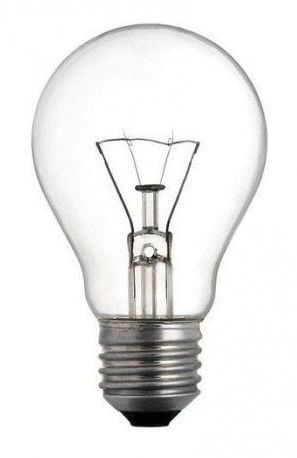
\includegraphics[width=0.5\textwidth]{Rysunek1.jpg}
  \caption{Żarówka tradycyjna}
  \label{Rys.1.1.}
\end{figure}

\section*{Światło żarówki}

Światło uzyskiwane z żarówek jest światłem zbliżonym do słonecznego i cechuje się dobrym wskaźnikiem oddawania barw oglądanych w tym świetle przedmiotów, świeci cały czas jednakowo, nie powodując efektu stroboskopowego. Widmo światła emitowanego przez żarówkę jest ciągłe, o niższej temperaturze barwowej (bardziej żółte) niż słoneczne. Temperatura barwowa światła emitowanego przez żarówkę wynosi ok. 2700 K. Wadą żarówek jest ich mała skuteczność świetlna, wynosząca zazwyczaj około 12 (od 8 do 16) lumenów/wat (niektóre mają sprawność poniżej 6 lumenów/wat), a także niska trwałość[a][b]. Żarówka wykorzystuje ok. 5% energii na światło widzialne, a reszta energii jest tracona w emisji ciepła co doskonale odzwierciedla rozkład widmowy promieniowania żarówki. Widać na nim wyraźnie, że żarówka emituje znaczną część promieniowania w zakresie podczerwieni.

\section*{Żarówka próżniowa}

Skuteczność świetlna żarówki zależy od temperatury żarnika. W miarę zwiększania temperatury żarnika szybko zwiększa się szybkość parowania wolframu, wskutek czego następuje tworzenie się przewężeń drutu wolframowego, zwiększone nagrzewanie się drutu w tym miejscu i w końcu przepalanie się żarnika. Wolfram odparowany z żarnika osadza się na bańce w postaci ciemnego nalotu, który pochłania część światła emitowanego przez żarnik. Z tych względów w żarówkach próżniowych (w bańce panuje próżnia) temperatura żarnika nie powinna przekraczać 2600 K.

\section*{Żarówka gazowana}

W celu zmniejszenia szybkości parowania wolframu, do wnętrza bańki wprowadza się gaz obojętny, powszechnie stosuje się argon z domieszką azotu. Wskutek zmniejszenia szybkości parowania wolframu żarnik żarówek gazowanych może pracować z wyższą temperaturą w wyniku czego uzyskuje się bielsze światło oraz większą skuteczność świetlną. Wprowadzenie gazu do wnętrza bańki powoduje, że część mocy doprowadzonej do żarnika jest odprowadzana poprzez gaz. Są to straty, które zależą między innymi od długości żarnika. Wykonanie żarnika w postaci skrętki, lub podwójnej skrętki powoduje skrócenie żarnika i obniżenie tych strat. Stosuje się też w miejsce argonu, gazy o mniejszym przewodnictwie cieplnym – krypton (żarówka kryptonowa) i jeszcze lepszy ksenon (żarówka ksenonowa). Jednak ich ceny (szczególnie ksenonu) są wysokie, co ogranicza ich stosowanie.

\section*{Żarówka halogenowa}

W żarówkach halogenowych do wnętrza bańki wprowadzony jest oprócz gazu obojętnego halogen, najczęściej jod. Halogen tworzy związek chemiczny z wolframem (parami wolframu w bańce i na ściankach bańki), związek ten krąży wraz z gazem w bańce, a w temperaturze panującej blisko żarnika rozpada się na wolfram i jod. W rezultacie tej reakcji następuje przenoszenie cząstek wyparowanego wolframu z bańki na żarnik. Proces ten nazywa się halogenowym cyklem regeneracyjnym. Występowanie tego cyklu pozwala zwiększyć temperaturę żarnika do około 3200 K, zatem żarówki halogenowe cechują się jeszcze wyższą skutecznością świetlną (do 18 lumenów/wat). Z uwagi na to, że podczas pracy żarnika o tak wysokiej temperaturze nagrzewają się również pozostałe elementy żarówki halogenowej (szczególnie bańka szklana, która może osiągnąć temperaturę nawet 527-827°C), bańkę halogenu wykonuje się z żaroodpornego szkła kwarcowego. Jej wymiary zostały też znacząco pomniejszone, co gwarantuje stabilność, a z kolei ciśnienie gazu zostało zwiększone, co spowolniło szybkość parowania wolframu.

\begin{figure}[ht]
  \centering
  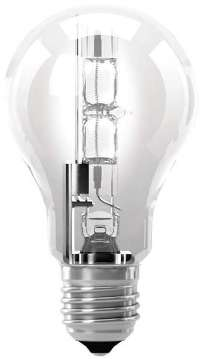
\includegraphics[width=0.5\textwidth]{Rysunek2.jpg}
  \caption{Żarówka halogenowa}
  \label{Rys.1.2.}
\end{figure}

Podane temperatury pracy żarnika odnoszą się do standardowych lamp, dla których przewidziano średni czas pracy 1000 godzin. Czasami, w sytuacjach gdy wymagane jest uzyskanie światła bardziej zbliżonego do światła dziennego, np. na planie zdjęciowym, stosuje się żarówki pracujące z wyższą temperaturą żarnika (w podręcznikach fotografii i kinematografii określane jako „żarówki przewoltowane”), trwałość tych lamp jest znacznie mniejsza, choć w praktyce można ją wydłużyć poprzez regulację napięcia: podczas ustawiania planu zdjęciowego (co trwa czasem kilka godzin) oprawy oświetleniowe zasila się 40-50% napięcia znamionowego, podając pełne napięcie tylko w momencie wykonywania zdjęć, czyli przez kilka do kilkunastu minut.

\chapter{ŚWIETLÓWKI}

\section*{Wstęp}

Niskoprężna lampa rtęciowa zwana potocznie świetlówką jest lampą wyładowczą (fluorescencyjnym źródłem światła), w której światło emitowane jest przez luminofor wzbudzony przez promieniowanie ultrafioletowe powstałe wskutek wyładowania jarzeniowego w rurze wypełnionej gazem. Tego typu wytwarzanie światła jest nazywane fotoluminescencją.

Prace nad zbudowaniem lampy zaczęły się w latach 30-tych XX wieku. Badaniami luminescencji zajmowali się wybitni fizycy, w Polsce był to Stefan Pieńkowski. Pierwszą w świecie świetlówkę (emitującą bladozielone światło), stworzył w 1935 roku Arthur Compton z General Electric, a w 1939 zaprezentował zestaw świetlówek na wystawie w Nowym Jorku.

\begin{figure}[ht]
  \centering
  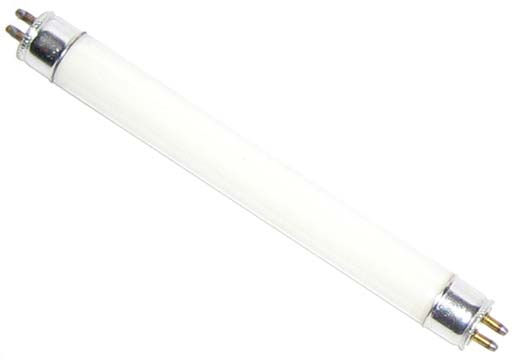
\includegraphics[width=0.5\textwidth]{Rysunek3.jpg}
  \caption{Świetlówka}
  \label{Rys.1.1.}
\end{figure}

\section*{Konstrukcja}

Świetlówka jest to lampa elektryczna mająca najczęściej kształt rury, pokrytej od wewnątrz luminoforem, wypełniona parami rtęci i argonem, w której źródłem świecenia jest promieniowanie widzialne emitowane przez warstwę luminoforu pokrywającego wewnętrzną powierzchnię rury. Wyładowania zachodzące pomiędzy elektrodami wolframowymi zabudowanymi przy końcach rury wytwarzają głównie niewidzialne promieniowanie ultrafioletowe o długości fali ok. 254 nm. Odpowiednio dobrane luminofory przetwarzają to promieniowanie na promieniowanie widzialne o pożądanej barwie światła (dzienne, chłodnobiałe, białe, ciepłobiałe, a nawet – głównie do celów dekoracyjnych – różnokolorowe, np. zielone, niebieskie, żółte, czerwone itp.).

Bańka świetlówki wykonana jest ze szkła zwykłego sodowo-wapniowego domieszkowanego tlenkiem żelaza w celu kontroli transmisji promieniowania ultrafioletowego. Rodzaj zastosowanego luminoforu w świetlówce decyduje o skuteczności świetlnej , wskaźniku oddawania barw CRI=Ra i temperaturze barwowej. Typowa charakterystyka widmowa świetlówki kompaktowej pokazuje, że w jej widmie występują linie rezonansowe rtęci z zakresu widzialnego (405, 436, 546, 579nm) oraz widmo ciągłe luminoforu (z maksimum w zakresie barwy czerwonej).

Poza świetlówkami prostymi (liniowymi), istnieją również świetlówki kołowe, U-kształtne oraz świetlówki kompaktowe (nazywane potocznie "żarówkami" energooszczędnymi), zintegrowane z układem zapłonowym i stabilizującym. Świetlówki takie mogą być wkręcane w miejsce tradycyjnych żarówek, ponieważ mają taki sam gwint, jak żarówka.

\section*{Odmiany konstrukcyjne}

Ze względu na stosowane luminofory, świetlówki można podzielić na:

\begin{itemize}
\item standardowe z luminoforami halofosforanowymi,
\item trójpasmowe z luminoforami wąskopasmowymi,
\item z luminoforami wielopasmowymi.
\end{itemize}

\noindent
Do zasilania świetlówek używane są dwa układy stabilizacyjno-zapłonowe:

\begin{itemize}
\item tradycyjny, ze statecznikiem magnetycznym (dławikiem), i zapłonnikiem (starterem),
\item elektroniczny.
\end{itemize}

\chapter{LEDy}

\section*{Wstęp}

W technice świetlnej przełom XX i XXI wieku daje się zaobserwować jako nadzwyczaj intensywna ekspansja półprzewodnikowych źródeł światła. Najbardziej znaczący rozwój dokonał się w odniesieniu do diod elektroluminescencyjnych, które od ang. Light Emitting Diodes są znane na rynku techniki świetlnej pod nazwą LED. Lampa LED (zwana potocznie "żarówką LED") jest to źródło światła zbudowane z diod elektroluminescencyjnych, umieszczone w obudowie pozwalającej zastosować je w oprawie oświetleniowej przeznaczonej dla żarówek.

\section*{Zasada działania}

Mechanizm generowania światła (fotonów) przez diody LED oparty jest na zjawisku elektroluminescencji. Jest to zjawisko przejścia elektronu ze stanu wzbudzonego do stanu podstawowego, co wiąże się z rekombinacją promienistą elektronu z dziurą, czyli z tzw. anihilacją i emisją energii w postaci fotonu. Dzięki najnowszej technologii wytwarzania związków półprzewodnikowych i możliwości regulacji składu procentowego poszczególnych pierwiastków tworzących materiał, można wytworzyć diodę emitującą praktycznie dowolną barwę światła (oprócz białej, bo, jak wiadomo, światło białe jest mieszaniną barw podstawowych – czerwonej, niebieskiej i zielonej).

\section*{Żarówki LED - białe}

Barwę białą w typowych żarówkach LED-owych otrzymuje się obecnie metodą hybrydową, gdzie jako diodę podstawową stosuje się diodę niebieską. Część jej promieniowania konwertowana jest przez jedną warstwę żółtego luminoforu, które następnie miesza się z resztą niezaabsorbowanego światła. W tym przypadku występuje mieszanie barwy żółtej i niebieskiej. Dzięki temu uzyskano białą diodę łatwą w wykonaniu, o prostym obwodzie zasilającym i charakteryzującą się brakiem szczątkowego promieniowania ultrafioletowego. 

Na rysunku poniżej przedstawiono charakterystyki widmowe dwóch diod elektroluminescencyjnych różniących się temperaturą barwową, która daje wrażenie światła białego zimnego (temperatura barwowa 6500K) i ciepłego (temperatura barwowa 3200K lub 2700K). W widmie tym występuje maksimum w zakresie barwy niebieskiej, odpowiadające widmu diody oraz maksimum w zakresie barwy o dłuższej długości fali odpowiadające świeceniu luminoforu. Jak widać widmo to jest zbliżone swoim wyglądem do widma źródła żarowego, w przeciwieństwie do widma świetlówki.

\begin{figure}[ht]
  \centering
  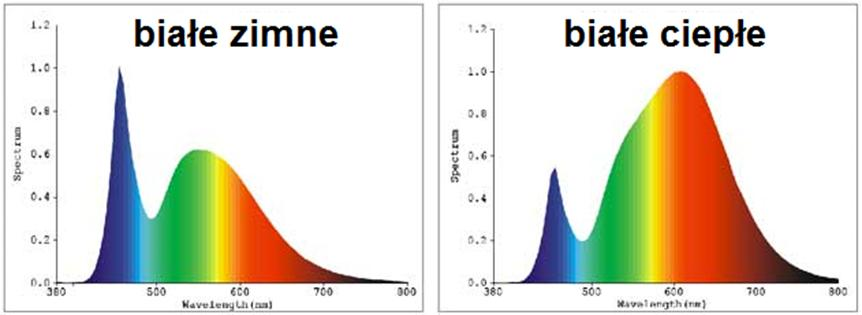
\includegraphics[width=0.5\textwidth]{Rysunek4.jpg}
  \caption{Widma promieniowania dwóch diod różniących się temperaturą barwową.}
  \label{Rys.3.1.}
\end{figure}

\section*{Żarówki LED – za zmianą barwy tzw. LED RGB}

Barwę białą w żarówkach LED-owych można również uzyskać innym sposobem, który jednocześnie umożliwia sterowanie emitowanymi przez takie źródło światła barwami. Jest to po prostu mieszanie trzech barw podstawowych (RGB-emitowanych przez osobne diody). Ponadto jest to najbardziej wydajne rozwiązanie, ponieważ na wyjściu takiego układu uzyskuje się sumę promieniowania ze wszystkich diod. Umożliwia ono uzyskanie szerokiego spektrum temperatury barwowej bieli oraz wysokiego współczynnika oddawania barw (na przykład poprzez dodanie dodatkowych diod, turkusowej i/lub bursztynowej). 

Metoda mieszania barw jednak nie jest doskonała. Głównymi wadami są niemożność idealnego wymieszania kolorów oraz szczególna wrażliwość diod czerwonych na zmianę parametrów zasilania oraz temperaturę otoczenia. Otrzymane światło, jeżeli w obudowie nie zaplanowano wydajnego rozpraszacza, charakteryzuje się różowawą poświatą. Natomiast w niestabilnych warunkach może wystąpić migotanie czerwonej diody, co przenosi się na złą jakość całego wyjściowego promieniowania.

\section*{Zalety i wady żarówek LED}

Do zalet diodowych źródeł światła zaliczyć można długi czas życia diody, który określa okres, po którym jasność diody obniży się do 70% (użyteczny czas życia) lub 50% (połowiczny czas życia). W przypadku LED-ów podaje się średnio wartość 100000 godzin pracy. W tym ujęciu zaletą LED-ów w porównaniu z innymi źródłami światła jest fakt, że jeżeli nie zniszczy się diody umyślnie lub nie podłączy jej w kierunku zaporowym, to nie nastąpi jej gwałtowne zaprzestanie działania (jak to się dzieje przy zastosowaniu na przykład żarówek czy lamp wyładowczych). Inną zaletą jest wysoka sprawność 100 lm/W, przy czym nie jest to jeszcze wartość graniczna. Diody LED nie marnują energii, która w przypadku innych źródeł światła emitowana jest jako promieniowanie podczerwone – ciepło. 

Co więcej niska cena eksploatacyjna daje zwrot inwestycji polegającej na wymianie tradycyjnego oświetlenia żarowego na lampy LED. Oszczędności osiągane na każdej wymienionej żarówce wynoszą (przy korzystaniu średnio przez 5 godzin) około 50 zł/rok w przypadku żarówki 60-watowej (odpowiednik to ok. 10-watowa lampa LED) i ok. 90 zł/rok dla 100-watowej (ok. 15-watowa lampa LED).

Źródła LED-owe charakteryzują się wysokim współczynnikiem oddawania barw, który dla najlepszych diod osiąga wartość CRI > 95. Diody LED mają bardzo krótkie czasy włączania (100 ns) i wyłączania (200 ns). W przeciwieństwie do lamp wyładowczych można je szybko włączać i wyłączać, i z powrotem włączać, bez zauważalnej zwłoki. Dzięki temu źródła te mogą również, bez żadnych dodatkowych urządzeń, imitować efekt stroboskopowy.

Zaletą lamp LED jest brak szkodliwego dla ludzkiego wzroku i skóry, a także dla dzieł sztuki promieniowania ultrafioletowego (UV) charakterystycznego dla świetlówek kompaktowych zawierających szkodliwą rtęć.
Wadą lamp LED jest inna charakterystyka widmowa niż naturalnego światła dziennego. Przy wyborze źródła światła należy zatem zwracać uwagę na opis lampy LED – np. "ciepła biała" i "zimna biała," co związane jest z temperatura barwową, zużycie energii oraz współczynnik oddawania barw CRI.

\tableofcontents

\listoffigures

\end{document}
